\documentclass[11pt, a4paper]{article}
\usepackage{sectsty}
\usepackage{graphicx}
\usepackage{amsmath}
\usepackage{amssymb}
\usepackage{setspace}
\usepackage{tasks}
\usepackage{graphicx}
\usepackage{float}
\usepackage{comment}
\usepackage{listings}
\usepackage[utf8]{inputenc}
\usepackage{amsfonts}
\usepackage{gensymb}
\usepackage{multicol}
\usepackage{tabularx}
\usepackage{tikz}
\newcommand{\myvec}[1]{\ensuremath{\begin{pmatrix}#1\end{pmatrix}}}
\let\vec\mathbf

\newcommand{\mydet}[1]{\ensuremath{\begin{vmatrix}#1\end{vmatrix}}}
\providecommand{\brak}[1]{\ensuremath{\left(#1\right)}}
\providecommand{\lbrak}[1]{\ensuremath{\left(#1\right.}}
\providecommand{\rbrak}[1]{\ensuremath{\left.#1\right)}}
\providecommand{\cbrak}[1]{\ensuremath{\left\{#1\right\}}}
\providecommand{\sbrak}[1]{\ensuremath{{}\left[#1\right]}}
\providecommand{\norm}[1]{\left\lVert#1\right\rVert}
\providecommand{\abs}[1]{\left\vert#1\right\vert}

\title{ Math computing}
\author{ Yaswanth }
\date{\today}

\begin{document}
\vspace{-\baselineskip}
\maketitle

\section*{NCERT 9.7.1.5}

\textbf{This question is from class 9 ncert chapter 7.triangles}
\begin{enumerate}
    \item Line $l$ is the bisector of an angle $\angle A$ and $B$ is any point on $l$. $BP$ and $BQ$ are perpendiculars from $B$ to the arms of $\angle A$. Show that:
%
\begin{enumerate}
    \item $\triangle  APB \cong \triangle AQB$  
    \item $BP$ = $BQ$ or $B$ is equidistant from the arms of $\angle A$.
 \end{enumerate}
\end{enumerate}
\begin{figure}[H]
    \centering
    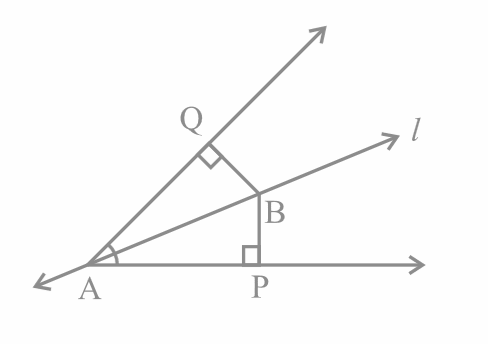
\includegraphics[width=1\columnwidth]{fig_mc.png}
    \caption{$\triangle AQB \hspace{12pt} and \hspace{12pt} \triangle APB$}
    \label{fig:math_comp1}
\end{figure}
\pagebreak
\textbf{Construction steps:}
%
\begin{enumerate}
\item
\begin{enumerate}

\item Let point $A$ be the reference point whose coordinates are at origin. 
\begin{align}
\vec{A} &= \myvec{0 \\ 0}
\end{align}

\item Let the distance between point $A$ and $B$ be $x$ ,and also considering the point $B$ on same axis .
\begin{align}
	\norm{A-B} &= x 
\end{align}

\item So,the coordinates of point $B$ be,
\begin{align}
\vec{B} &= \myvec{x \\ 0}
\end{align}

\item Let the coordinates of point $P$ be,
\begin{align}
\vec{P} &= \myvec{ a \\ b} 
\end{align}

\item And,let the coordinates of point $Q$ be,
\begin{align}
\vec{Q} &= \myvec{ c \\ d} 
\end{align}

\item Let assume the distance between point $A$ and $P$ be $r$ ,and let the line $AB$ makes an angle $ \theta $ anticlock wise with line $AP$.
\begin{align}
	\norm{A-P} &= r \\
\angle PAB &= \theta
\end{align}

\item Now the coordinates of point $P$ will be,
\begin{align}
\vec{P} &= \myvec{ a \\ b } = \myvec{r \cos \theta \\ -r \sin \theta} 
\end{align}

\item Similarly , let assume the distance between point $A$ and $Q$ also be $r$ , and the line $AB$ makes an angle $\theta$ clock wise with line $AQ$.
\begin{align}
	\norm{A-Q} &= r \\
\angle QAB &= \theta 
\end{align}

\item Now the coordinates of point $Q$ will be,
\begin{align}
\vec{Q} &= \myvec{ c \\ d } = \myvec{r \cos \theta \\ r \sin \theta} 
\end{align}

% Coordinates with generalised parameters
\item Now the coordinates of $A$,$B$,$P$,$Q$ are ,
\begin{align}
\vec{A} &= \myvec{0 \\ 0},\,
\vec{B} &= \myvec{x \\ 0} ,\,
\vec{P} &= \myvec{r \cos \theta \\ -r \sin \theta} ,\,
\vec{Q} &= \myvec{r \cos \theta \\ r \sin \theta} 
\end{align}

\item Let assume, 
\begin{align}
	x &= 5 \\
	r &=4 \\
	\theta &= 30 \degree
\end{align}

\item on substituting the values ,
\begin{align}
\vec{A} &= \myvec{0 \\ 0},\,
\vec{B} &= \myvec{5 \\ 0} ,\,
\vec{P} &= \myvec{4 \cos 30 \degree \\ -4 \sin 30 \degree } ,\,
\vec{Q} &= \myvec{4 \cos 30 \degree \\ 4 \sin 30 \degree } 
\end{align}

\item on calculating we get  ,
\begin{align}
\vec{A} &= \myvec{0 \\ 0},\,
\vec{B} &= \myvec{5 \\ 0} ,\,
\vec{P} &= \myvec{ 3.464101 \\ -2 } ,\,
\vec{Q} &= \myvec{3.464101  \\ 2 } 
\end{align}
Joining these points forms the required figure

\end{enumerate}
\end{enumerate}

\begin{figure}[H]
    \centering
    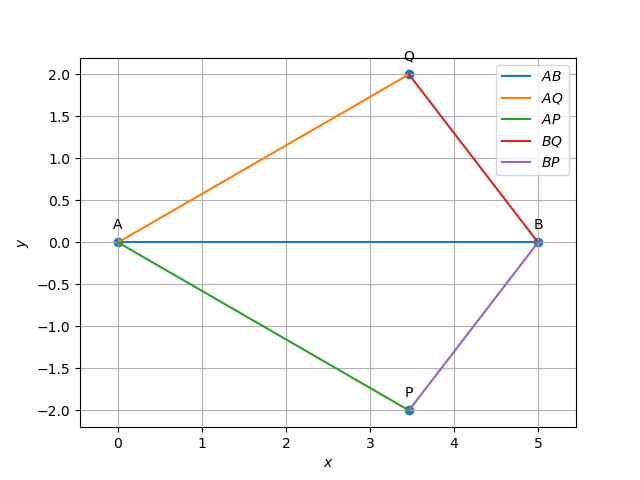
\includegraphics[width=\columnwidth]{fig_mat_comp.png}
    \caption{$\triangle APB \hspace{12pt} and \hspace{12pt} \triangle AQB$}
    \label{fig:math_comp2}
\end{figure}

\end{document}
